\section{Resultados}
% En esta sección se presentan los resultados obtenidos durante la implementación y prueba de los distintos módulos desarrollados: el sistema de reconocimiento de colores, el piano electrónico, la cerradura con contraseña y el control del plotter. Cada módulo fue verificado individualmente en simulación y en montaje físico, registrando su funcionamiento y las principales observaciones.

\subsection{Resultados por módulo}

\subsubsection{\textbf{Plotter}}---
% Explicá cómo se verificó el movimiento (por ejemplo, ejecución de trayectorias simples o figuras predefinidas).

% Mostrá fotos o diagramas de movimiento, si tenés.

% Comentá observaciones: velocidad, precisión, limitaciones por USART.

% 💬 Ejemplo:

% El plotter ejecutó correctamente trayectorias lineales y circulares generadas desde un script en Python. Se comprobó que, al reducir la tasa de envío por USART, la respuesta del sistema fue más fluida y sin interrupciones perceptibles.

\subsubsection{\textbf{Colores}}---
% Mostrá la tabla o los valores obtenidos por el LDR para cada color calibrado.

\begin{table}[H]
\centering
\caption{Valores de referencia RGB para cada color calibrado.}
\begin{tabular}{lccc}
\toprule
\textbf{Color} & \textbf{R} & \textbf{G} & \textbf{B} \\
\midrule
Morado      & 216 & 157 & 274 \\
Rojo        & 206 & 149 & 262 \\
Amarillo    & 196 &  99 & 105 \\
Verde       & 272 & 192 & 152 \\
Azul Claro  & 151 & 153 & 122 \\
Violeta     & 253 & 275 & 338 \\
Blanco      & 110 &  93 &  91 \\
\bottomrule
\end{tabular}
\label{tab:color_ref}
\end{table}

% Incluí una figura de la tira LED mostrando el color detectado o el ángulo del servo.

\begin{figure}[H]
    \centering
    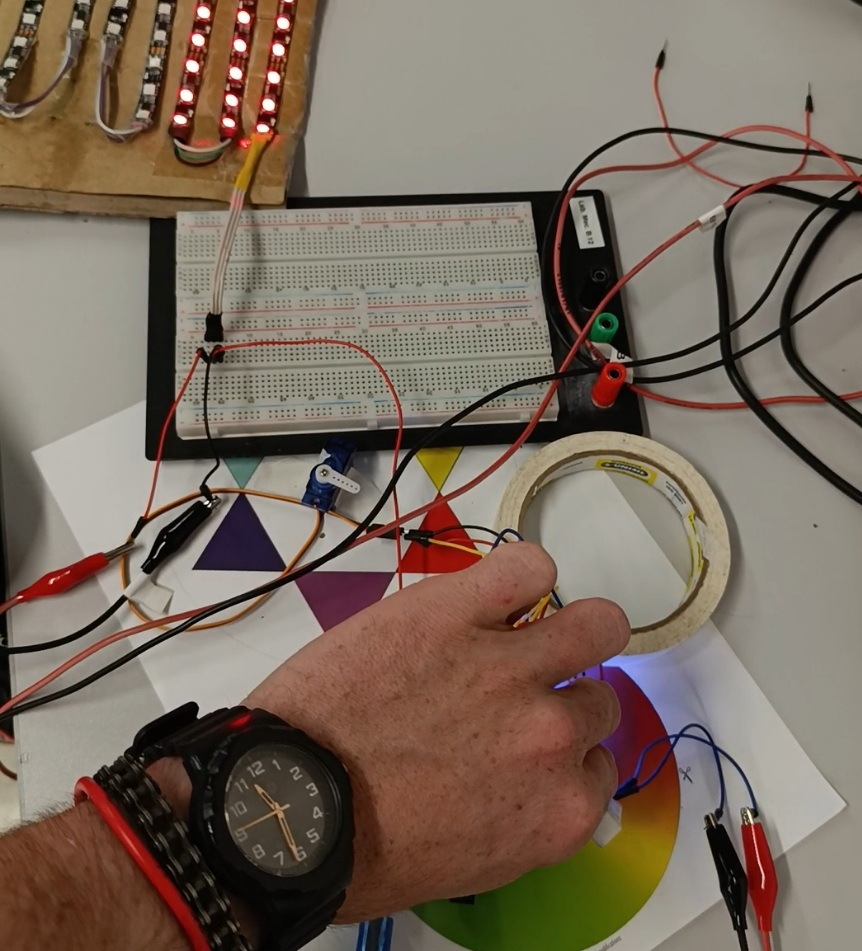
\includegraphics[width=0.9\columnwidth]{anexos/colores/EvidenciaFuncionamiento.jpg}
    \caption{Identificación de color efectiva. Fuente: elaboración própia}
    \label{fig:color_evidencia}
\end{figure}


% Mencioná el comportamiento: estabilidad, sensibilidad a la luz ambiente, etc.

% Estabilidad frente a consumo
Utilizando una fuente externa el sistema es considerablemente estable
Como el servomotor posee un pico de consumo en momentos de arranque, si este es alimentado solamente con el voltaje del Arduino, algunos colores se volvían inestables y creaba fallas en la medición, haciendo un ciclo de retroalimentación.

% Estabilidad a luz ambiental
Otra consideración fue que el sistema también es dependiente en cierta medida a la cantidad de luz ambiental del lugar en el que se encuentre. La misma tira de LEDs al iluminarse a veces causaba falsas medidas, se solventó esto bloqueando la luz de la tira hacia el sensor.

% Delay frente a USART
También, al implementar la impresión de datos a través de USART, se observó una ralentización considerable del funcionamiento del programa debido al tiempo que le tomaba enviarse a los datos para cada ciclo. Al quitar esta funcionalidad el sistema lograba un aumento significativo en su velocidad de operación.

% ----------------------------------------- RAMBLINGS

% Reconocer colores
% Como se reconoce un color
% Un color se puede descomoner en otros colores
% Colores primarios
% Colores CYMK
% Colores RGB
% Un LDR no puede medir componentes
% Un LDR solo mide luz reflejada
% Si iluminamos con luz blanca el LDR mide la cantidad de luz blanca que rebota
% Seria como tener vision en blanco y negro
% Algunos colores serian dificiles de identificar

% Si iluminamos con otro color el LDR ve la cantidad de luz que refleja de ese color
% Si iluminamos con rojo, luego verde, y luego azul el LDR puede identificar 
% colores con 3 grados de libertad como el ojo humano.

% Se utiliza un led RGB para iluminar con estos colores

% El LDR no responde la misma manera a todos los tipos de luz. 
% Los valores medidos no se van a correlacionar de manera directa
% Con las componentes tradicionales de cada color.
% Ademas de que existen variaciones de emision de luz entre los mismos colores del led

% Sin embargo es suficiente si lo calibramos antes

% Utilizando un divisor de voltaje se conecta el ldr a un pin analogico del arduino

% Se ilumina con rojo verde y azul para cada color y se recopilan los valores medidos por el ADC

% Se mapean los 6 colores de la hoja para tomar como referencias.

% Para determinar el color el cual el LDR esta apuntando
% se calcula cual es el valor más próximo tomando
% en cuenta los 3 componentes como ejes de libertad
% realizando un calculo de distancia cartesiana.
% A2 + B2 + C2 = D2

% En este caso rojo verde y azul representan un eje en un espacio tridimensional. 
% Los colores calibrados representan vectores. Y el vector de medición se 
% mueve a lo largo de todo este espacio adquiriendo diferentes valores rgb.

% De manera ciclica se mide la distancia del vector medicion con respecto 
% al resto de vectores mapeados para identificar cual es el vector que 
% mas se aproxima al vector medición

% Problemas
% Como medir colores con presicion
% Como reconocer colores precalibrados
% Como controlar un servomotor
% Como controlar una tira LED

% Funcionaldiades
% Salida de info por USART
% Color indicado por angulo en servomotor
% Color indica



\subsubsection{\textbf{Piano}}---

% Mostrá capturas de los menús USART, las canciones reproducidas o las frecuencias generadas.

% Explicá el uso de interrupciones para reproducir melodías sin detener el programa.

% Comentá si el sonido fue limpio, si hubo desfase, o cómo responden los botones.

% 💬 Ejemplo:

% El piano electrónico logró reproducir correctamente las melodías “Cha-La Head-Cha-La” y “Still Alive”. Cada nota se generó a partir del temporizador 0 configurado en modo CTC. La reproducción simultánea de pistas A y B mostró un leve desfase tras varios segundos de ejecución, atribuible a pequeñas diferencias en el conteo de interrupciones.

% ---------------------------- RAMBLINGS

% Sonido
% Que es el sonido
% Ondas
% Difrentes tipos de ondas
% Como hacemos sonido
% Buzzer
% Onda cuadrada
% Como funciona el buzzer
% Piezo
% Como lo hacemos sonar con el atmega
% Variacion de frecuencia
% Como hacemos otro sonido
% Cambiamos la frencuencia
% Como hacemos musica
% Teoria musical basica
% Mapeo de notas
% Una nota es una frecuencia
% Una frecuencia durante un tiempo es una nota
% Como guardamos musica
% Nota musical: frencuencia, tiempo encendido, tiempo apagado
% Secuencia de notas musicales --- musica
% La musica se compone de varios instrumentos en paralelo
% Como reproducimos varios instrumentos
% Evitar polling --- Utilizar timers

% Problemas
% Como reproducir sonido
% Como representar una nota musical
% Como reproducir pistas en paralelo

% Funcionalidades
% Control por USART
% Piano fisico




\subsubsection{\textbf{Cerradura}}---

% Mostrá el flujo de la interfaz (mensajes en LCD, ingreso de contraseña, cambio de clave, activación de alarma).

% Si podés, mostrás una tabla con los estados de la máquina y qué hace cada uno.

% Comentá observaciones de funcionamiento en simulación vs físico.

% 💬 Ejemplo:

% El sistema respondió correctamente al ingreso de contraseñas válidas e inválidas. Tras tres intentos fallidos, se activó la alarma visual y sonora. El cambio de contraseña fue exitoso y persistió tras apagar el microcontrolador, confirmando la correcta escritura en EEPROM. En PicSimLab, el teclado dejó de responder tras reiniciar, pero en el hardware físico el funcionamiento fue estable.

% -------------------------- RAMBLINGS

% Cerradura
% Que tiene que hacer
% Candado cerrado
% Contraseña correcta
% Candado abierto
% Sino 3 veces alarma

% Cambiar contraseña
% Contra actual
% Contra nueva
% Guaradado

% Contraseñas tienen que ser entre 4 y 6 digitos

% Problema
% Una interfaz de usuario
% Que es una interfaz
% Entradas y salidas
% El usuario hace algo y la interfaz muestra algo
% Es la parte del programa o sistema que se encarga
% de hablar con el usuario.
% Diferentes acciones muestran o hacen diferentes cosas
% Maquina de estados --- Transiciones de estado.
% Problema: Reproducir sonidos, hacer debouncing, manejar alarmas, pantalla LCD. 
% No existen suficientes timers
% Solucion: tareas o tasks
% Utilizar un contador de tiempo interno de 32 bits
% junto con un solo timer para manejar tareas en paralelo

% La tarea se ejecuta rapidamente en el main y compara el timepo que paso con 
% el tiempo especificado para una acción especifica.

% Un solo timer. Muchos delays sin polling.

% Otro problema
% Contraseña debe ser guardada aunque el sistema esté apagado
% Solucion EEPROM
% Funcionamiento de la eeprom
% limitaciones de escritura de EEPROM
% Como leer
% Como escribir

% Otro problema
% Teclado matricial
% Usa menos pines, uno por fila uno por columna
% Como identificar botones presionados
% Respuesta multiplexado
% Filas funcionan como salidas
% Columnas funcionan como entradas (pullup interno)
% Al solamente apagar una fila a la vez (0) 
% va a hacer que el pin de esa columna se vuelva 0
% Funcion retorna el caracter que representa esa fila y columna
% Listo.











\subsection{Evidencias gráficas y mediciones}
% Capturas del LCD, fotos del montaje, gráficos de lectura ADC, diagramas de flujo, etc.

% Si mediste tiempos, tensiones o corrientes, ponelos en tabla o gráfico simple.

\subsection{Comentario general}
% Un breve cierre que enlace con la sección de conclusiones:

	% En general, todos los módulos cumplieron los objetivos planteados. Se lograron lecturas estables, respuestas correctas y sincronización entre las distintas tareas, demostrando la integración de hardware y software en un entorno embebido con recursos limitados.
